\subsection{Arten von Machine Learning}

Der wichtigste und komplizierteste Teil beim machinellem Lernen, ist die Kunst einem Computer das selbständige Lernen beizubringen, dabei orientiert man sich am Lernprozess eines Menschens. Dazu besteht es eine Vielzahl an Ansätzen und zu den bekanntesten gehören:

\begin{itemize}
    \item Supervised Learning
    \item Unsupervised Learning
    \item Reinforcement Learning
\end{itemize}

Um diese Ansätze nachvollziehen zu können, muss man zuerst die meschliche Intelligent verstehen, oder genauer gessagt die Frage ''Wie lernt das menschliche Gehirn?''. 

\subsubsection{Menschliche Ürsprünge vom Machine Learning}

Ein Neugeborenes kommt mit circa 100 Milliarden Neuronen auf die Welt, diese sind jedoch nur schwach miteiander verknüpft. Mithilfe des Lernens werden diese Verbindungen gestärkt und das Kind kann Vorgehensweisen besser 
verstehen und neue Erkenntnisse gewinnen.

\begin{figure}[ht]
    \centering
    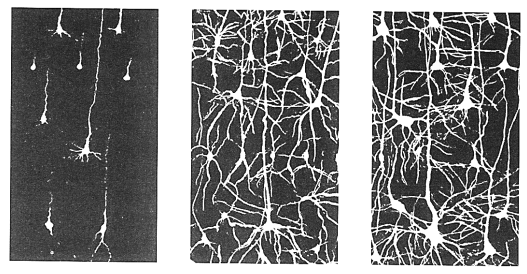
\includegraphics[scale=0.8]{sections/machine-learning/images/neuronale-netze.png}
    \caption{Vernetzungen nach der Geburt, nach 3 Monaten und nach 15 Monaten}
\end{figure}
%https://www.uni-wuerzburg.de/fileadmin/06000060/04_Fort-_und_Weiterbildungen_Lehrkraefte/Herbsttagungen/Herbsttagung_2016/20161006_WS_04_Neurobiologie.pdf

Die gegenwärtige Neurobiologie, definiert das Lernen als vielschichtigen Prozess, welcher Neuronenverbänder plastisch miteinander verbindet undso bilden sich Netzwerke und System aus Neuroenen. Umso mehr Verbindungen entstehen und mit dem Wiederholen des Gelernten gestärkt werden, desto besser kann das Erlernte aufgerufen werden und mit dem bereits existierenden Vorwissen kombiniert werden.

Mithilfe einem zwecksentfermdeten, morphologischem Kasten, auch Zwicky-Box genannt, kann man das menschliche Gehirn vereinfacht darstellen. Dabei gibt die erste Spalte ausgewählte Merkmale an und die darauf folgenden Spalten eine  weitere Ausspägung vom Merkmal in der selben Zeile. Die große Anzahl der Ausprägungen ermöglicht später breite Auswahl an Ausgägen der Zwicky-Box. 

\begin{table}[ht]
    \centering
    \resizebox{.7\textwidth}{!}{
    \begin{tabular}{|l|l|l|l|}
    \hline
        \textbf{Merkmal}  & \multicolumn{3}{c|}{ \textbf{Ausprägungen}}   \\ \hline
        Augenfarbe & Blau & Grün & Braun  \\ \hline
        Haarfarbe & Blond & Brünett & Schwarz  \\ \hline
        Frisur & Lang & Glaze & Kurz  \\ \hline
        Gesichtsform & Schmal & Rund & Oval  \\ \hline
        Nase & Klein & Groß & Flach  \\ \hline
        Brille & Ja & Nein & ~ \\ \hline
    \end{tabular}}
    \caption{Beispiel einer Zwicky-Boy}
\end{table}

In dieser Zwicky-Box wurden Merkmale eines Menschens aufgezählt. Um einen Ausgang darzustellen wird für jedes Merkmal eine Ausprägung ausgewählt und mit einer Linie verbunden, damit man eine Ausprägung von anderen unterscheiden kann. In diesem Beispiel wird die Linie durch verschiedenen Farben ersetzt.

\begin{table}[ht]
    \centering
    \resizebox{.7\textwidth}{!}{
        \begin{tabular}{|l|l|l|l|}
        \hline
        \textbf{Merkmal}  & \multicolumn{3}{c|}{ \textbf{Ausprägungen}}   \\ \hline
        Augenfarbe & \cellcolor{blue!25}Blau & Grün & Braun  \\ \hline
        Haarfarbe & Blond & \cellcolor{blue!25}Brünett & Schwarz  \\ \hline
        Frisur & \cellcolor{blue!25}Lang & Glaze & Kurz  \\ \hline
        Gesichtsform & \cellcolor{blue!25}Schmal & Oval & Rund  \\ \hline
        Brille & \cellcolor{blue!25}Ja & Nein & ~ \\ \hline
        \end{tabular}
    }
    \caption{Beispiel einer Ausprägung}
    \label{fig:zwicky-box}
\end{table}

Jede eingefärbte Zelle kann man als ''aufleuchtendes'' Neuron interpretieren, wenn man versucht das Geschlecht einer fremden Person zu identifizieren. Jedoch lernt man durch dieses ''Aufleuchten'' nicht, da man das eigentliche Geschlecht der Person nicht kennt und man daher keine Verbindungen aufbauen kann. Durch das Kennenlernen von Personen und Merken derer Ausprägungen werden diese oben genannten Neuronenverbindungen aufgebaut, welche später genutzt werden, um das Geschlecht einer fremden Person festzustellen. Diese Art von Lernen ist ein sehr schneller und effektiver Prozess, der mit vielen Nachteilen kommt, denn genau auf diesem Weg werden Vorurteile gebildet. Anhand eines Beispieles: Die meisten würden die obigen Werte aus der Zwicky-Box als Frau wahrnehmen, jedoch könnte jede kleinste Änderung am Aussehen diese Wahrnehmung beeinflussen.

\begin{table}[ht]
    \centering
    \resizebox{.7\textwidth}{!}{
    \begin{tabular}{|l|l|l|l|}
    \hline
        \textbf{Merkmal}  & \multicolumn{3}{c|}{ \textbf{Ausprägungen}}   \\ \hline
        Augenfarbe & \cellcolor{blue!25}Blau & Grün & Braun  \\ \hline
        Haarfarbe & Blond & \cellcolor{blue!25}Brünett & Schwarz  \\ \hline
        Frisur & \cellcolor{blue!25}Lang & Glaze & Kurz  \\ \hline
        Gesichtsform & \cellcolor{blue!25}Schmal & Oval & Rund  \\ \hline
        Brille & \cellcolor{blue!25}Ja & Nein & ~ \\ \hline
        ~ & ~ & ~ & ~  \\ \hline
        Ergebnis: & Frau & ~ & ~ \\ \hline
        Sicherheit: & 70\% & ~ & ~ \\ \hline
    \end{tabular}}
    \caption{Ergebnis einer Ausprägung}
\end{table}

Da das Aussehen im Beispiel dem Aussehen von Bekannten in gewissen Merkmalen ähnelt, kann man mit einer Wahrscheinlichkeit von 70\% sagen, dass es sich um eine Frau handelt. Desto mehr Personen man kennt, umso besser und genauer werden die Ausprägungen dem Geschlecht zugeteilt und die Sicherheit wird erhöht. 

In dem Fall, dass ein Merkmal nicht erkennbar ist, wird versucht das beste Ergebnis zu finden, jedoch wird die Sicherheit drastisch fallen.

\subsubsection{Supervised Learning}

Hierbei werden gelabelte (daher auch ''supervised'' oder im deutsche überwacht) Datensätze genutzt, um Daten zu klassifizieren oder Vorhersagen genau wie möglich aufzustellen. Diese Art von Lernen kann man in zwei Typen aufteilen:

\paragraph{Klassifizierungs} Probleme verwenden Algorithmen, um Daten einer bestimmten Kategorie zuzuteilen. Oft gibt es nur zwei Kategorien wie zum Beispiel Hund/Katze oder Ja/Nein, jedoch gibt es auch Fälle wo eine Vorhersage mit einer Wahrscheinlichkeit zwischen 0 und 1 getroggen wird. Weiteres gibt es auch Situationen, wo zwischen einer großen Menge an Kategorien ausgewählt wird, zum Beispiel bei der Erkennung von handschriftlichen Ziffern, in diesem Beispiel würde es zehn Möglichkeiten geben.

Zu diesen ''überwachten'' Algorithmen gehören Lineare Diskriminanzanalysen, Support Vector Machines (SVM), Random Forests und Entscheidungsbäume \cite{SL:online}.

\subparagraph{Entscheidungsbäume,} oder im Englischem Decision Trees, sind Visualisierungen von Entscheidungswegen, oder auch aufgefächerte Zwicky-Boxen, die die Verbidungen visualisieren.

\begin{figure}[ht]
    \centering
    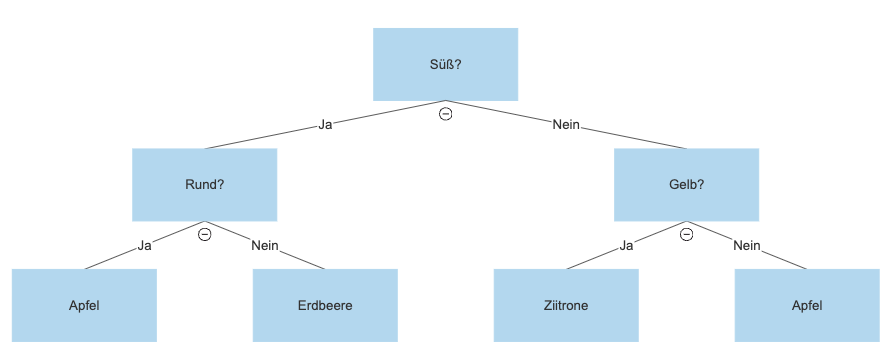
\includegraphics[scale=0.4]{sections/machine-learning/images/decision-tree.png}
    \caption{Decision Tree an dem Beispiel von \ref{fig:zwicky-box}}
\end{figure}

In diesem Beispiel sieht dieser Entscheidungsbaum noch sehr lesbar aus, jedoch ändert sich dies, wenn Entscheidungen dargestellt werden, bei denen es auf die Nachkommastelle ankommt und wenn die Kategorien sehr schwer differenzierbar sind. Bei dem Supervised Learning erstellt das Programm selbstständig einen Entscheidungsbaum, indem es Muster oder Zusammenhänge findet und analysiert. Nach vielem Lernen kann dieser Entscheidungsbaum optimiert werden und unnötige Verbindungen können entfernt werden. Jedoch kann es auch passieren, dass durch Zufälle unberechenbare Verbindungen gefunden werden, dieses Problem wird ''Overfitting''. 

\subparagraph{Overfitting} bedeutet, dass ein Modell perfekt an die Testdaten angepasst ist, jedoch bei unbekannten Daten falsche Verbindungen aufbauen könnte und dadurch falsche Ergebnisse vorhergesagt werden. 

\paragraph{Regressionen,} Erstellung einer kontinuierlichen Funktion mithilfe von Werten, die auf oder nahe an der Funktion liegen, sind hilfreich, wenn anstatt diskreten Werten kontinuierliche Werte, wie zum Beispiel die Größe einer Person, festgestellt werden sollen. Dazu gehören lineare Regressionen und logistische Regressionen.

\subsubsection{Unsupervised Learning}

Beim Unsupervised Learning, oder Unüberwachtes Lernen, erzeugt Verbidungen ohne genauere Informationen über den Testdatensatz. Dabei muss das Programm selbst Gruppen definieren und dann die übergebenen Daten in diese Gruppen zuordnen.

\paragraph{Clustering} ist einer der beliebtesten Varaiante, um selbstständig Gruppen zu erstellen. Dabei wird jeder Datensatz als Punkt in ein Koordiantensystem mit beliebig vielen Dimesionen eingetragen. Eine Achse stellt ein Attribut dar und je nach Ausprägung ist der Punkt mehr oder weniger vom Ursprung entfernt. 

\begin{figure}[ht]
    \centering
    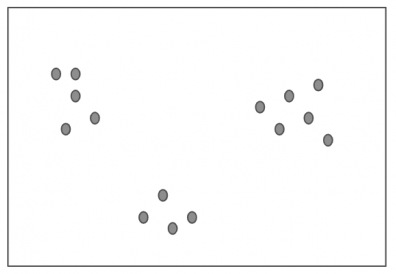
\includegraphics[scale=0.8]{sections/machine-learning/images/unclustered-data.png}
    \caption{Unkategorisierte Daten}
    \label{fig:unclustered-data}
\end{figure}
%https://datascience.eu/de/maschinelles-lernen/clustering-algorithmen-und-ihre-bedeutung-beim-maschinellen-lernen-2/

Auch für das menschliche Auge ist es möglich dieses Beispiel \ref{fig:unclustered-data} in Haufen oder Klumpen zusammenzufassen, genau das gleiche macht ein Programm mit Clustern. Die Interpretation dieser Gruppen muss jedoch wieder durch Menschen erfolgen, da ein Computer nicht im Stande dazu ist, dieser Cluster einer Kategorie zuzuteilen.

Diese Vorgehensweise wird oft in sehr komplizierte Einsatzbereiche genutzt, und daher ist es oft sehr schwer differenzierbare Cluster zu erstellen. Der Prozess, solche Cluster zu definieren, basiert darauf die Punkte so zu gruppieren, dass der Abstand in diesem Cluster klein ist und zu anderen Clustern groß.

\begin{figure}[ht]
    \centering
    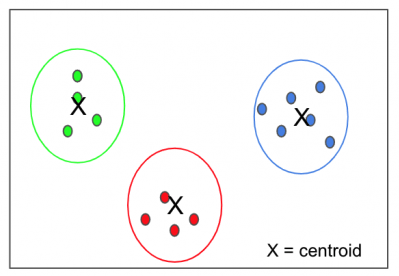
\includegraphics[scale=0.8]{sections/machine-learning/images/clustered-data.png}
    \caption{Kategorisierte Daten}
    \label{fig:clustered-data}
\end{figure}

\subsubsection{Reinforcement Learning}

Das Reinforcement Learning oder das beschränkte/verstärkte Lernen wird oft mit dem Konzept ''Learning by doing'' verglichen, da es sich weniger auf das Ergebnis fokussiert und mehr auf Aktionen oder Vorgängen. Ein Beispiel für diese Vorgehensweise aus der Sicht eines Schülers ist das Üben vor einer Matheschularbeit. Wird während dem Üben ein Fehler gemacht, merkt man sich das Problem und passt sein Verhalten / seinen Rechenweg so an, dass dieser Fehler nicht mehr vorkommt. Die nennt man auch negative Verstärkung. 

Dahingegen führen richtige Ergebnisse oder erwarteten Reaktionen zu positiven Verstärkungen und man versucht dieses Verhalten zu wiederholen.

Durch negative und positive Verstärkungen wird das Verhalten verbessert, um den besten Weg zum Ziel zu finden. Bei komplexen Systemen kann dies selbstständig vom Programm gemacht werden, jedoch bei simpleren kann es geschehen, dass ein unnötig komplizierter Weg gefunden wird. In diesen Fällen schaut ein Supervisor dem Programm ''über die Schulter''.